% ============================================================
% TEMPLATE LaTeX — Relatório de Inteligência INTEIA (Dark Premium)
% Compilar com: xelatex relatorio_inteia.tex
% ============================================================
\documentclass[a4paper,11pt]{article}

% === PACOTES ===
\usepackage[top=20mm,bottom=18mm,left=22mm,right=18mm]{geometry}
\usepackage{fontspec}
\usepackage{xcolor}
\usepackage{graphicx}
\usepackage{tikz}
\usepackage{tabularx}
\usepackage{booktabs}
\usepackage{enumitem}
\usepackage{fancyhdr}
\usepackage{titlesec}
\usepackage{multicol}
\usepackage{hyperref}
\usepackage{pagecolor}
\usepackage{afterpage}
\usepackage{calc}
\usepackage{eso-pic}
\usepackage{setspace}

% === CORES INTEIA ===
\definecolor{void}{HTML}{050608}
\definecolor{obsidian}{HTML}{0a0b0f}
\definecolor{carbon}{HTML}{111318}
\definecolor{graphite}{HTML}{1a1d26}
\definecolor{slate}{HTML}{252832}
\definecolor{gold}{HTML}{c9952a}
\definecolor{gold2}{HTML}{e8b84b}
\definecolor{gold3}{HTML}{f5d07a}
\definecolor{crimson}{HTML}{c0392b}
\definecolor{crimson2}{HTML}{e74c3c}
\definecolor{emerald}{HTML}{1a7a4a}
\definecolor{emerald2}{HTML}{27ae60}
\definecolor{cobalt}{HTML}{1a4a8a}
\definecolor{cobalt2}{HTML}{2980b9}
\definecolor{amber}{HTML}{d68c1a}
\definecolor{textcolor}{HTML}{eeeae0}
\definecolor{muted}{HTML}{8a8680}
\definecolor{dim}{HTML}{4a4845}
\definecolor{border}{HTML}{1e2030}

% === FUNDO ESCURO ===
\pagecolor{void}
\color{textcolor}

% === FONTES (requer xelatex) ===
% Fallback: se não tiver as fontes instaladas, usa Latin Modern
\IfFontExistsTF{Cormorant Garamond}{
  \setmainfont{Cormorant Garamond}[
    UprightFont=*-Regular,
    BoldFont=*-Bold,
    ItalicFont=*-Italic,
    BoldItalicFont=*-BoldItalic,
  ]
}{
  \setmainfont{Latin Modern Roman}
}
\IfFontExistsTF{Outfit}{
  \setsansfont{Outfit}[
    UprightFont=*-Regular,
    BoldFont=*-Bold,
  ]
}{
  \setsansfont{Latin Modern Sans}
}
\IfFontExistsTF{JetBrains Mono}{
  \setmonofont{JetBrains Mono}[Scale=0.85]
}{
  \setmonofont{Latin Modern Mono}[Scale=0.85]
}

% === HYPERLINKS ===
\hypersetup{
  colorlinks=true,
  linkcolor=gold2,
  urlcolor=gold2,
  citecolor=gold,
  pdfauthor={INTEIA — Inteligência Estratégica},
}

% === CABEÇALHO E RODAPÉ ===
\pagestyle{fancy}
\fancyhf{}
\renewcommand{\headrulewidth}{0pt}
\fancyfoot[L]{{\fontsize{6}{7}\selectfont\color{dim}\texttt{INTEIA · Inteligência Estratégica · inteia.com.br}}}
\fancyfoot[R]{{\fontsize{6}{7}\selectfont\color{dim}\texttt{Página \thepage}}}
\fancyfoot[C]{}

% === SIDEBAR DOURADA (faixa esquerda em todas as páginas) ===
\AddToShipoutPictureBG{%
  \AtPageLowerLeft{%
    \color{gold}\rule{1.5mm}{\paperheight}%
  }%
}

% === TÍTULOS ===
\titleformat{\section}
  {\Large\bfseries\color{gold2}}
  {\textcolor{gold}{\thesection}}
  {1em}
  {}
  [\vspace{-0.5em}{\color{border}\hrule height 0.4pt}]

\titleformat{\subsection}
  {\normalsize\bfseries\color{textcolor}}
  {\textcolor{gold}{\thesubsection}}
  {0.8em}
  {}

\titleformat{\subsubsection}
  {\small\ttfamily\uppercase\color{gold}}
  {}
  {0em}
  {}

\titlespacing*{\section}{0pt}{2.5em}{1.2em}
\titlespacing*{\subsection}{0pt}{1.8em}{0.8em}
\titlespacing*{\subsubsection}{0pt}{1.5em}{0.6em}

% === COMANDOS UTILITÁRIOS ===

% Chip/badge
\newcommand{\chip}[1]{%
  \fcolorbox{border}{carbon}{\fontsize{6}{7}\selectfont\texttt{\color{muted}#1}}%
}
\newcommand{\chipgold}[1]{%
  \fcolorbox{gold}{carbon}{\fontsize{6}{7}\selectfont\texttt{\color{gold2}#1}}%
}
\newcommand{\chipred}[1]{%
  \fcolorbox{crimson}{carbon}{\fontsize{6}{7}\selectfont\texttt{\color{crimson2}#1}}%
}

% KPI box
\newcommand{\kpi}[3][gold2]{%  #1=cor, #2=valor, #3=label
  \begin{tikzpicture}
    \fill[carbon] (0,0) rectangle (4.2,2);
    \fill[#1] (0,1.97) rectangle (4.2,2);
    \node[anchor=west,text=#1] at (0.3,1.2) {\fontsize{20}{22}\selectfont\bfseries #2};
    \node[anchor=west,text=muted] at (0.3,0.4) {\fontsize{6}{7}\selectfont\texttt{\uppercase{#3}}};
  \end{tikzpicture}%
}

% Box com borda lateral (altura dinâmica — texto longo não transborda)
\newcommand{\inteiabox}[3][gold]{%  #1=cor borda, #2=label, #3=texto
  \par\vspace{0.8em}%
  \noindent\fcolorbox{carbon}{carbon}{%
    \hspace{-\fboxsep}%
    \textcolor{#1}{\rule{2pt}{\dimexpr\baselineskip*3+\fboxsep*2\relax}}% borda lateral mínima
    \hspace{0.4em}%
    \begin{minipage}{\dimexpr\linewidth-2\fboxsep-2\fboxrule-0.8em}%
      {\fontsize{6}{7}\selectfont\ttfamily\color{muted}\uppercase{#2}}\\[0.4em]%
      {\sffamily\fontsize{9}{12}\selectfont\color{textcolor}#3}%
    \end{minipage}%
  }%
  \par\vspace{0.5em}%
}

% Veredicto
\newenvironment{veredicto}{%
  \par\vspace{1.5em}%
  \noindent\fcolorbox{gold}{carbon}{%
  \begin{minipage}{\dimexpr\linewidth-2\fboxsep-2\fboxrule}%
  \centering\vspace{1em}%
  {\fontsize{6}{7}\selectfont\texttt{\color{gold}\uppercase{Veredicto Consolidado}}}\\[0.8em]%
}{%
  \vspace{1em}%
  \end{minipage}}%
  \par\vspace{1.5em}%
}

% Separador de seção
\newcommand{\pagesep}[1]{%
  \par\vspace{2em}%
  \noindent{\color{border}\hrule height 0.3pt}%
  \vspace{0.4em}%
  \begin{center}{\fontsize{6}{7}\selectfont\texttt{\color{dim}\uppercase{#1}}}\end{center}%
  \vspace{0.4em}%
  {\color{border}\hrule height 0.3pt}%
  \par\vspace{1.5em}%
}

% Quadrante SWOT (altura dinâmica — texto longo não transborda)
\newcommand{\swotquad}[3]{%  #1=cor, #2=titulo, #3=items
  \fcolorbox{carbon}{carbon}{%
    \begin{minipage}[t]{0.44\linewidth}%
      \vspace{0pt}%
      {\color{#1}\rule{\linewidth}{2pt}}\\[0.3em]%
      {\fontsize{7}{8}\selectfont\ttfamily\color{#1}\uppercase{#2}}\\[0.5em]%
      {\sffamily\fontsize{8.5}{11}\selectfont\color{muted}#3}%
      \vspace{0.5em}%
    \end{minipage}%
  }%
}

% === DOCUMENTO ===
\begin{document}
\thispagestyle{empty}

% ============================================================
% CAPA
% ============================================================
\begin{tikzpicture}[remember picture,overlay]
  % Fundo capa
  \fill[obsidian] (current page.south west) rectangle (current page.north east);
  % Grade decorativa
  \foreach \x in {0,1,...,20} {
    \draw[gold,opacity=0.035] (\x*0.6-1,0) -- (\x*0.6-1,30);
  }
  \foreach \y in {0,1,...,50} {
    \draw[gold,opacity=0.035] (-1,\y*0.6) -- (22,\y*0.6);
  }
  % Barra lateral dourada
  \fill[gold] (current page.south west) rectangle ([xshift=1.5mm]current page.north west);
  % Glow superior direito
  \shade[inner color=gold,outer color=obsidian,opacity=0.08] (current page.north east) circle (8cm);
\end{tikzpicture}

\vspace*{3cm}

% Logo + brand
\noindent
\begin{minipage}{0.6\linewidth}
  % Se tiver o logo PNG, descomentar:
  % 
\includegraphics[height=3.5cm]{logo_inteia_transparent.png}\\[0.8em]
  {\fontsize{14}{16}\selectfont\texttt{\color{gold}\uppercase{INTEIA}}}\\[0.2em]
  {\fontsize{7}{8}\selectfont\texttt{\color{muted}Inteligência Artificial Estratégica}}\\
  {\fontsize{7}{8}\selectfont\texttt{\color{gold}Preditiva Eleitoral}}
\end{minipage}%
\hfill
\begin{minipage}{0.3\linewidth}
  \raggedleft
  \fcolorbox{crimson2}{void}{\fontsize{6}{7}\selectfont\texttt{\color{crimson2}\uppercase{Confidencial}}}
\end{minipage}

\vspace{3cm}

% Eyebrow
{\fontsize{7}{8}\selectfont\texttt{\color{gold}\uppercase{%
  % ← PREENCHER: contexto do relatório
  Relatório de Inteligência · Março 2026%
}}}

\vspace{1.5em}

% Título principal
{\fontsize{38}{40}\selectfont\bfseries\color{textcolor}%
  % ← PREENCHER: título do relatório
  Título do\\Relatório \textcolor{gold2}{\textit{Estratégico}}%
}

\vspace{0.8em}

% Subtítulo
{\fontsize{18}{22}\selectfont\itshape\color{muted}%
  % ← PREENCHER: subtítulo
  Subtítulo com contexto político%
}

\vspace{2em}

% Regra dourada
{\color{gold}\rule{3cm}{1.5pt}}

\vspace{1.5em}

% Descrição
{\sffamily\fontsize{10}{14}\selectfont\color{muted}%
  % ← PREENCHER: descrição
  Análise integrada com 16 metodologias convergentes, simulações com agentes sintéticos
  e teoria dos jogos aplicada ao cenário político.%
}

\vspace{2em}

% Chips
\chipred{Confidencial}\quad
\chipgold{Confiança: 0,XX}\quad
\chip{Março 2026}\quad
\chip{n = XXXX agentes}\quad
\chip{Igor M. Vasconcelos · PhD}

\vfill

% Footer da capa
\noindent{\color{border}\hrule height 0.3pt}
\vspace{0.6em}
\noindent
\begin{minipage}{0.5\linewidth}
  {\fontsize{6}{7}\selectfont\texttt{\color{dim}\uppercase{Versão}}}\\
  {\fontsize{7}{8}\selectfont\texttt{\color{muted}v1.0 Final}}
\end{minipage}%
\hfill
\begin{minipage}{0.5\linewidth}
  \raggedleft
  {\fontsize{6}{7}\selectfont\texttt{\color{dim}\uppercase{Metodologias}}}\\
  {\fontsize{7}{8}\selectfont\texttt{\color{muted}16 convergentes + MAD}}
\end{minipage}

% Número decorativo
\begin{tikzpicture}[remember picture,overlay]
  \node[anchor=south east,opacity=0.04,text=gold] at ([xshift=-2cm,yshift=3cm]current page.south east) {\fontsize{120}{120}\selectfont\bfseries 16};
\end{tikzpicture}

\newpage

% ============================================================
% CONTEÚDO (preencher seções abaixo)
% ============================================================

\section{Resumo Executivo}

\begin{veredicto}
  {\fontsize{16}{20}\selectfont\bfseries\color{gold2}%
    % ← PREENCHER: veredicto principal em 1 frase
    [Veredicto principal aqui]%
  }\\[0.8em]
  {\fontsize{8}{10}\selectfont\texttt{\color{muted}%
    % ← PREENCHER: fluxo causal
    Causa → Mecanismo → Consequência → Recomendação%
  }}\\[1em]
  % Stats
  \begin{tabular}{ccc}
    {\fontsize{22}{24}\selectfont\bfseries\color{gold2} XX\%} &
    {\fontsize{22}{24}\selectfont\bfseries\color{gold2} 0,XX} &
    {\fontsize{22}{24}\selectfont\bfseries\color{gold2} N/N} \\
    {\fontsize{6}{7}\selectfont\texttt{\color{muted}\uppercase{P(vitória)}}} &
    {\fontsize{6}{7}\selectfont\texttt{\color{muted}\uppercase{Confiança}}} &
    {\fontsize{6}{7}\selectfont\texttt{\color{muted}\uppercase{Convergência}}} \\
  \end{tabular}
\end{veredicto}

% Aviso crítico
\inteiabox[crimson2]{Aviso Crítico}{%
  % ← PREENCHER: aviso ou ressalva principal
  [Texto do aviso crítico]%
}

\section{Metodologia}

% Pills das 16 metodologias
\noindent
\chip{Nash 2×2}\;
\chip{Stackelberg}\;
\chip{Bayesiano}\;
\chip{Shapley/Core}\;
\chip{Dilema do Prisioneiro}\;
\chip{Sinalização Spence}\;
\chip{Eleitores Sintéticos}\;
\chip{Consultores Lendários}\;
\chip{Parlamentares}\;
\chip{SWOT}\;
\chip{PESTEL}\;
\chip{Stakeholders}\;
\chip{MCDA}\;
\chip{Matriz de Risco}\;
\chip{Process Tracing}\;
\chip{Frame Analysis}

% ← ADICIONAR seções conforme o relatório:
% \section{A Crise}
% \section{Teoria dos Jogos}
% \section{Simulações com Agentes Sintéticos}
% \section{SWOT Eleitoral}
% \section{Plano de Ação}
% \section{Monitor de Imprensa}
% \section{Autores}

\vfill

% ============================================================
% RODAPÉ FINAL
% ============================================================
\noindent{\color{border}\hrule height 0.3pt}
\vspace{0.5em}
\begin{center}
  {\fontsize{7}{8}\selectfont\texttt{\color{gold}\uppercase{INTEIA}} \color{dim}· Inteligência Estratégica}\\[0.3em]
  {\fontsize{6}{7}\selectfont\color{dim}\texttt{%
    SHN Quadra 2 Bloco F, Sala 625/626 — Brasília/DF · inteia.com.br · igor@inteia.com.br%
  }}\\[0.2em]
  {\fontsize{5.5}{6}\selectfont\color{dim}\texttt{© 2026 INTEIA. Todos os direitos reservados.}}
\end{center}

\end{document}
